\chapter{Linear Programming}
In this chapter we introduce the concept of linear programming. Most proofs will be omitted but proofs and more in depth explanations can be found in ~\cite{vanderbei2015linear}
\section{The structure of a linear program (LP)}
In a linear program we want to maximize or minimize a given linear function $z:\R^n \rightarrow \R$ subject to a number of linear inequalities or equalities $g_i:\R^n \rightarrow \R$ with $g_i(x_1,...,x_n)\geq b_i$,$g_i(x_1,...,x_n)\leq b_i$ or $g_i(x_1,...,x_n)= b_i$. The function, $z$, that we want to optimise is called the \textbf{objective} and the set of inequalities are called the \textbf{constraints}. A general linear problem is written:
\begin{align}\label{lpform}
\begin{array}{ll@{}ll}
\text{min/max} &z(x_1,...,x_n)&\\
\text{s.t.} &g_1(x_1,...,x_n) \textbf{ ordRel } b_1,&\\
&\vdots&\\
&g_m(x_1,...,x_n) \textbf{ ordRel } b_m&\\
&\text{where each \textbf{ordRel} can be }\leq,\geq \text{ or } =&
\end{array}
\end{align}

\begin{example}\label{lpex}
A maths student wants to save money on his diet while still remaining healthy. To stay healthy his diet must contain at least $b_1=6$ units of protein, $b_2=15$ units of carbs, $b_3=5$ units of fat and $b_4=7$ units of vitamins.\\
He considers buying 3 food products with different nutritional values and prices: 
\begin{enumerate}
\item $x_1$ is a take away meal costing 5 and containing 3 units of protein, 3 units of carbs, 2 units of fat and 1 unit of vitamins.
\item $x_2$ is a vegetable costing 1 and containing 1 unit of protein, 2 units of carbs, 0 units of fat and 4 units of vitamins.
\item $x_3$ is a type of bread costing 2 and containing $\frac{1}{2}$ unit of protein, 4 units of carbs, 1 unit of fat and 0 units of vitamins.
\end{enumerate}
He then define an optimization problem minimizing the cost of food subject to getting the right nutrition
\begin{align}
\begin{array}{ll@{}ll}
\text{min} &5x_1+x_2+2x_3&\\
\text{s.t.} &3x_1+x_2+\frac{1}{2}x_3 \geq 6,&\\
&3x_1+2x_2+4x_3 \geq 15,&\\
&2x_1+x_3 \geq 5,&\\
&x_1+4x_2 \geq 7,&\\
&x_1,x_2,x_3 \geq 0,&\\
\end{array}
\end{align}
He finds the cheapest solution to be $x_1 = 1, x_2= \frac{3}{2},x_3 = 3$ and buys one take away meal, one and a half vegetable and three loafs of bread to a total cost of $12.5$.
\end{example}
\section{Feasible and optimal solutions}
\subsection{Feasibility}
Given a Linear problem on form \ref{lpform} any point of $\R^n$ such that all $m$ constraints are satisfied is called a feasible solution. The set of all these points is called the feasible set. In the case of \Cref{lpex} the feasible set is the set of all combinations of amounts of the different foods such that the nutritional requirements are met. If a problem has no feasible solutions, that problem is said to be infeasible. A feasibility problem is a special case in linear programming where our object function is constant and thus if any feasible solution exists, that solution is optimal.
\subsection{Optimal solutions}
A feasible solution $\textbf{x}_0 \in \R^n$ is said to be optimal if $z(\textbf{x}_0) \geq z(\textbf{x})$ (when maximizing) or $z(\textbf{x}_0) \leq z(\textbf{x})$ (when minimizing) for all feasible solutions $\textbf{x} \in \R^n$.\\
In some instances when feasible solutions exist, but no maximal (or minimal) solution exists the problem is said to be \textbf{unbounded}. In that case one or more variable in the objective can approach $\infty$ or $-\infty$ in a solution, all while the solution remains feasible and the objective value diverges.
\section{Convexity}
\begin{definition}\label{convex}
A set $X \in \R^n$ is said to be convex if for any two points $a, b \in X$ the straight line segment 
%$\{x|x=(1-t)a+tb,t\in [0,1]\}$
connecting $a$ and $b$ is entirely within $X$.
\end{definition}
\begin{theorem}
A feasible set of a linear program is convex
\begin{proof}
The feasible subset of $\R^n$ of an LP is exactly the intersection of all the half-spaces given by each constraint function where an equality is seen as two half spaces defined by two inequalities. \\
Since such half-spaces are convex and the intersection of convex sets is also convex, the entire feasible set is convex.
\end{proof}
\end{theorem}
\begin{definition}
An intersection of half spaces is known as a \textbf{convex polyhedron}. 
\end{definition}
\begin{definition}
A \textbf{face} of a polyhedron $P$ is a subset $\{x\in P:g(x)=b\}$ of the boundary of $P$ where $g(x) \geq b$ is some half-space containing the polyhedron. 
\end{definition}
\begin{definition}
An \textbf{extreme point} (vertex) of a convex polyhedron is a face consisting of a single point.
\end{definition}
\begin{lemma}\label{face}
Any face of a polyhedron $P\subset \R^n$ contains an extreme point of $P$ or is unbounded.
\iffalse
\begin{proof}
The intersection of two faces is itself a face of $P$ since the intersection is on the boundary and intersects the half-space defined by $g_1(x)+g_2(x)\geq b_1+b_2$ where $g_1(x) \geq b_1$ and $g_2(x) \geq b_2$ are the inequalities defining the half-spaces intersecting each of the two faces. Thus an extreme point is a face in itself and is contained in all faces that intersect in that point. If a face contains no extreme points it is unbounded on at least one coordinate, since at most $n-1$ of the half-spaces bounding $P$ intersect in any point of the face.
\end{proof}
\fi
\end{lemma}
\subsection{The Fundamental Theorem of Linear Programming}
\begin{theorem}\label{extreme point}
If a set $\mathcal{S}$ of optimal solutions to a given LP is non-empty, then some solution $s\in \mathcal{S}$ exists such that $s$ is in an extreme point in the feasible set.
\begin{proof}
Suppose that the given LP is a minimization problem. Suppose $\mathcal{S} =\{z(\textbf{x})= \zeta \}$ is the set of optimal solutions to the LP. Then by $\mathcal{S}$ being optimal, the half space $z(\textbf{x}) \leq \zeta$ contains the convex polyhedron $\mathcal{P}$ of the feasible space and $z(\textbf{x})= \zeta$ is a subset of the boundary.\\
Thus $\mathcal{S}$ is a face of $\mathcal{P}$ and by \Cref{face} it contains an extreme point.\\
The proof for maximization problems is analogous.
\end{proof}
\end{theorem}
\section{The geometric/graphical intuition}
From a geometric perspective the feasible region of an LP can be seen as a convex polyhedron encapsulated by the hyperplanes defined by each constraint function. The objective is a hyperplane that can be "pushed" orthogonally to either maximize or minimize a point of the plane such that it is contained in the feasible polyhedron.\\ 
In case of \Cref{lpex}, with three real variables, $x_1,x_2,x_3$ the polyhedron will be a polyhedron in $\R^3$ and the objective plane will be the plane defined by the linear equation $5x_1+x_2+2x_3 = \zeta $ where $\zeta $ is the value we want to minimize. 
\begin{figure}[H]
\centering
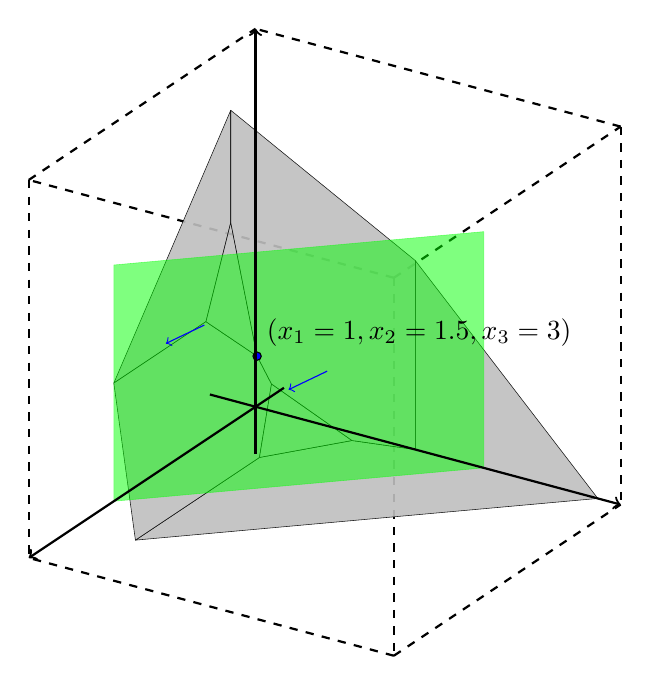
\begin{tikzpicture}[x  = {(0.9659cm,-0.25882cm)},
                    y  = {(-0.6cm,-0.4cm)},
                    z  = {(0cm,1cm)},
                    scale = 0.3,
                    color = {black}]
% style of faces
\tikzset{facestyle/.style={fill=black,draw=black,very thin,line join=round}}
% axis 
% coordinates
%x1>0
\coordinate (C1) at (0, 7/4, 53/4);
\coordinate (C2) at (0, 10, 5);
\coordinate (C3) at (0, 7/4, 17/2);
\coordinate (C4) at (0, 7/2, 5);
%x_2>0
\coordinate (C5) at (15, 0, 0);
\coordinate (C6) at (7, 0, 0);
\coordinate (C7) at (7, 0, 8);
%x3>0
%(C5) (C6)
\coordinate (C8) at (5/2, 25/2, 0);
\coordinate (C9) at (5/2, 15/4, 0);
\coordinate (C10) at (23/5, 3/5, 0);
%intersections
\coordinate (C11) at (17/11, 15/11, 21/11);
\coordinate (C12) at (1, 3/2, 3);%optimal
%objective plane
\coordinate (O1) at (10, 0, 0);
\coordinate (O2) at (10, 0, 10);
\coordinate (O4) at (0, 10, 0);
\coordinate (O3) at (0, 10, 10);

%box
\draw [black, dashed, thick] (16,16,0) -- (16,0,0);
\draw [black, dashed, thick] (16,16,0) -- (0,16,0);
\draw [black, dashed, thick] (16,0,16) -- (16,0,0);
\draw [black, dashed, thick] (16,0,16) -- (0,0,16);
\draw [black, dashed, thick] (0,16,16) -- (0,16,0);
\draw [black, dashed, thick] (0,16,16) -- (0,0,16);
\draw [black, dashed, thick] (16,16,16) -- (0,16,16);
\draw [black, dashed, thick] (16,16,16) -- (16,0,16);
\draw [black, dashed, thick] (16,16,16) -- (16,16,0);

%fill polyhedron-
%C1
\draw[fill=lightgray,draw=black,opacity=.9,very thin,line join=round]
 (C1) --
 (C2) --
 (C4) -- 
 (C3) -- cycle ;
 %C3
\draw[fill=lightgray,draw=black,opacity=.9,very thin,line join=round]
 (C5) --
 (C6) --
 (C7) --cycle ;
 %C4
\draw[fill=lightgray,draw=black,opacity=.9,very thin,line join=round]
  (C5) --
  (C6) --
  (C10)--
  (C9)--
  (C8)-- cycle ;
\draw[fill=lightgray,draw=black,opacity=.9,very thin,line join=round]
  (C8) --
  (C9) --
  (C11)--
  (C12)--
  (C4)--
  (C2)-- cycle ;
\draw[fill=lightgray,draw=black,opacity=.9,very thin,line join=round]
  (C10) --
  (C9) --
  (C11)-- cycle ;
\draw[fill=lightgray,draw=black,opacity=.9,very thin,line join=round]
  (C12) --
  (C3) --
  (C4)-- cycle ;
\draw[fill=lightgray,draw=black,opacity=.9,very thin,line join=round]
  (C7) --
  (C6) --
  (C10)--
  (C11)--
  (C12)--
  (C3)-- 
  (C1)--cycle ;
  
%objective:
\draw[fill=green,draw=green,opacity=.5,very thin,line join=round]
(O1)--
(O2)--
(O3)--
(O4)--cycle;

\draw[fill=blue] (C12) circle (0.5em)
	    node[above right] {$(x_1=1,x_2=1.5,x_3=3)$};
%C2
%\draw[fill=gray,draw=red,opacity=.8,very thin,line join=round]
% (A232) --
% (A242) --
% (A231) --
% (A241) --
% (A122) --cycle ;
\draw [blue, arrows = ->] (5,3,4) -- (3,2.5,2.5);
\draw [blue, arrows = ->] (-1,2,4) -- (-3,1.5,2.5);
%extreme points
\draw [black, thick, arrows = ->] (0,0,-2) -- (0,0,16);
\draw [black, thick, arrows = ->] (0,-2,0) -- (0,16,0);
\draw [black, thick, arrows = ->] (-2,0,0) -- (16,0,0);
\end{tikzpicture}
\caption{A graphical repressentation of \Cref{lpex}}
\end{figure}
\section{Matrix representation of an LP and Slack variables}
Since the objective function and the constraints of a linear program are all linear functions we can also write a linear program using matrix-vector products. \\
The objective can be written as the product of the vector of variables to be determined 
$\begin{bmatrix}x_{1} \\ x_{2} \\
\vdots \\
x_{n}
\end{bmatrix}=\textbf{x}$, and the transposed vector of coefficients $[c_1,c_2,...,c_n]=\textbf{c}^T$ of each $x_i$ in the objective.\\
Likewise the constraints can be written as the matrix-vector product of $\textbf{x}$ with a certain matrix, $A$.\\
Rewriting any $\leq$ constraint to $\geq$ in case of minimization or any $\geq$ to $\leq$ in case of maximization (the equality constraints can be written with two inequalities) we can write the linear program in it's \textit{canonical form}:
\begin{align}\label{canonicalMin}
\begin{array}{ll@{}ll}
\text{min} &\textbf{c}^T\textbf{x}&\\
\text{s.t.} &A\textbf{x} \geq \textbf{b},&\\
&\textbf{x} \geq 0,&\\
\end{array}
\end{align}
\begin{align}\label{canonicalMax}
\begin{array}{ll@{}ll}
\text{max} &\textbf{c}^T\textbf{x}&\\
\text{s.t.} &A\textbf{x} \leq \textbf{b},&\\
&\textbf{x} \geq 0,&\\
\end{array}
\end{align}
in case of \Cref{lpex} we write it on it's canonical form:
\begin{align}
\begin{array}{ll@{}ll}
\text{min} &[5,1,2]\begin{bmatrix}x_{1} \\x_{2} \\x_{3}\end{bmatrix}&\\
\text{s.t.} &\begin{bmatrix}3&2&1 \\12&2&4 \\7&0&2\\3&5&2\end{bmatrix}\begin{bmatrix}x_{1} \\x_{2} \\x_{3}\end{bmatrix} \geq \begin{bmatrix}5 \\10 \\5\\10\end{bmatrix},&\\
&\textbf{x} \geq 0,&\\
\end{array}
\end{align}
Much like how we made an LP on canonical form by manipulating the inequalities, we can also write any LP on it's \textit{standard form} 
\begin{align}
\begin{array}{ll@{}ll}
\text{max/min} &\textbf{c}^T\textbf{x}&\\
\text{s.t.} &A\textbf{x} = \textbf{b},&\\
&\textbf{x} \geq 0,&\\
\end{array}
\end{align}
by introducing a $1\times m$ vector, $\textbf{s}$, with one slack variable for each constraint and thus creating a new LP on standard form with the same solutions as the old one.
\begin{align}
\begin{array}{ll@{}ll}
\text{max} &\textbf{c}^T\textbf{x}&\\
\text{s.t.} &A\textbf{x}+\textbf{s} =\textbf{b},&\\
&\textbf{x,s} \geq 0,&\\
\end{array}
\end{align}
These forms and the concept of slack variables will come in handy later
\iffalse
\section{Duality}
Another important result in Linear programming is the concept of duality.
\begin{definition}
Given a maximization linear program on canonical form \ref{canonicalMax}
We define it's dual problem as the minimization problem:
\begin{align}\label{canonicalMaxDual}
\begin{array}{ll@{}ll}
\text{min} &\textbf{b}^T\textbf{y}&\\
\text{s.t.} &A^T\textbf{y} \geq \textbf{c},&\\
&\textbf{y} \geq 0,&\\
\end{array}
\end{align}
\end{definition}
\begin{theorem}
An optimal solution to a linear program on it's primal form is also optimal in the dual form
\begin{proof}
\todo{proof}
\end{proof}
\end{theorem}
\subsection{Weak and strong duality}
\fi
\section{Efficiency of solving an LP}
\subsection{The simplex method}
A popular algorithm for finding the optimal solution of LPs, taking advantage of the convexity of the feasible region and \Cref{extreme point} is the \textbf{Simplex method}. ~\cite{vanderbei2015linear}, where Theorem 3.4 also gives a proof of \ref{extreme point} using the simplex method, explains this further. The basic idea of the algorithm is to move from extreme point to extreme point of the feasible set and never return to an already visited solution. Thus the algorithm will find an optimal solution after at most the number of extreme points iterations. If a problem has $n$ variables and $m$ constraints, an upper bound of the number of iterations is 
\begin{align*}
\begin{pmatrix}
n+m\\m
\end{pmatrix}.
\end{align*} 
which is maximized when $n=m$. Thus we see that 
\begin{align*}
\frac{1}{2n}2^{2n}\leq\begin{pmatrix}
n+m\\m
\end{pmatrix}\leq 2^{2n}
\end{align*}
So the worst-case running time of the simplex method is exponential.
\subsection{Polynomial time algorithms}
Even though the simplex method is one of the most popular algorithms, the worst case runtime is exponential compared to the problem size. Other algorithms have however been introduced, which have a polynomial worst case runtime. In 1979 Leonid Khachiyan \cite{khachiyan1980polynomial} gave the first algorithm, the \textit{ellipsoid method}, proved to run in polynomial time later Narendra Karmarkar ~\cite{karmarkar1984new} gave a new, more efficient, algorithm also solving linear problems in polynomial time.
\\ Even though these algorithms have better worst case time complexity compared to the simplex method, they are often slower in practice. They do however show that linear programming is in $\mathcal{P}$.
\\\\ In the next chapter we will introduce Integer programming which is $\mathcal{NP}$-hard.